\appendix
\titleformat{\chapter}[display]
  {\normalfont\bfseries\centering\fontsize{16}{20}\selectfont}
  {PHỤ LỤC \thechapter}{0.4em}{\MakeUppercase}
\chapter{THÔNG TIN PHỤC VỤ PHIẾU ĐÁNH GIÁ}

\section{Thông tin sinh viên và đợt thực tập}

\noindent\begin{tabularx}{\textwidth}{>{\bfseries}p{5cm}X}
Họ và tên & \StudentName \\
MSSV & \StudentId \\
Lớp & \StudentClass \\
Ngày sinh & \StudentDob \\
Cơ quan thực tập & \CompanyName \\
Địa chỉ & \CompanyAddress \\
Thời gian & \InternshipPeriod \\
Người hướng dẫn & \CompanySupervisor \\
Đại diện xác nhận & \CompanyRepresentative, Phó Tổng giám đốc \\
\end{tabularx}

\section{Nội dung thực tập tóm tắt}

Tìm hiểu cơ cấu tổ chức và các lĩnh vực hoạt động của Công ty Cổ phần TECHPAL.
Khảo sát danh mục linh kiện điện tử và thiết bị tự động hóa công nghiệp. Tìm
hiểu phương pháp đọc mã linh kiện, datasheet và các tiêu chí kỹ thuật khi lựa
chọn thiết bị. Đối chiếu một số mã sản phẩm đại diện với tài liệu của nhà sản
xuất và xây dựng bảng kiểm kỹ thuật trước khi lựa chọn thiết bị. Xây dựng yêu
cầu và sơ đồ khối minh họa
cho hệ thống giám sát nhiệt độ tủ kỹ thuật. Tổng hợp kết quả, nhận xét nhược điểm và
đề xuất hướng hoàn thiện.

\chapter{MINH CHỨNG THỰC TẬP}

\section{Phiếu đánh giá quá trình thực tập}

Bản scan phiếu đánh giá do đơn vị tiếp nhận lập được trình bày trong Hình
\ref{fig:phieu-trang-1} và Hình \ref{fig:phieu-trang-2}.

\begin{figure}[H]
\centering
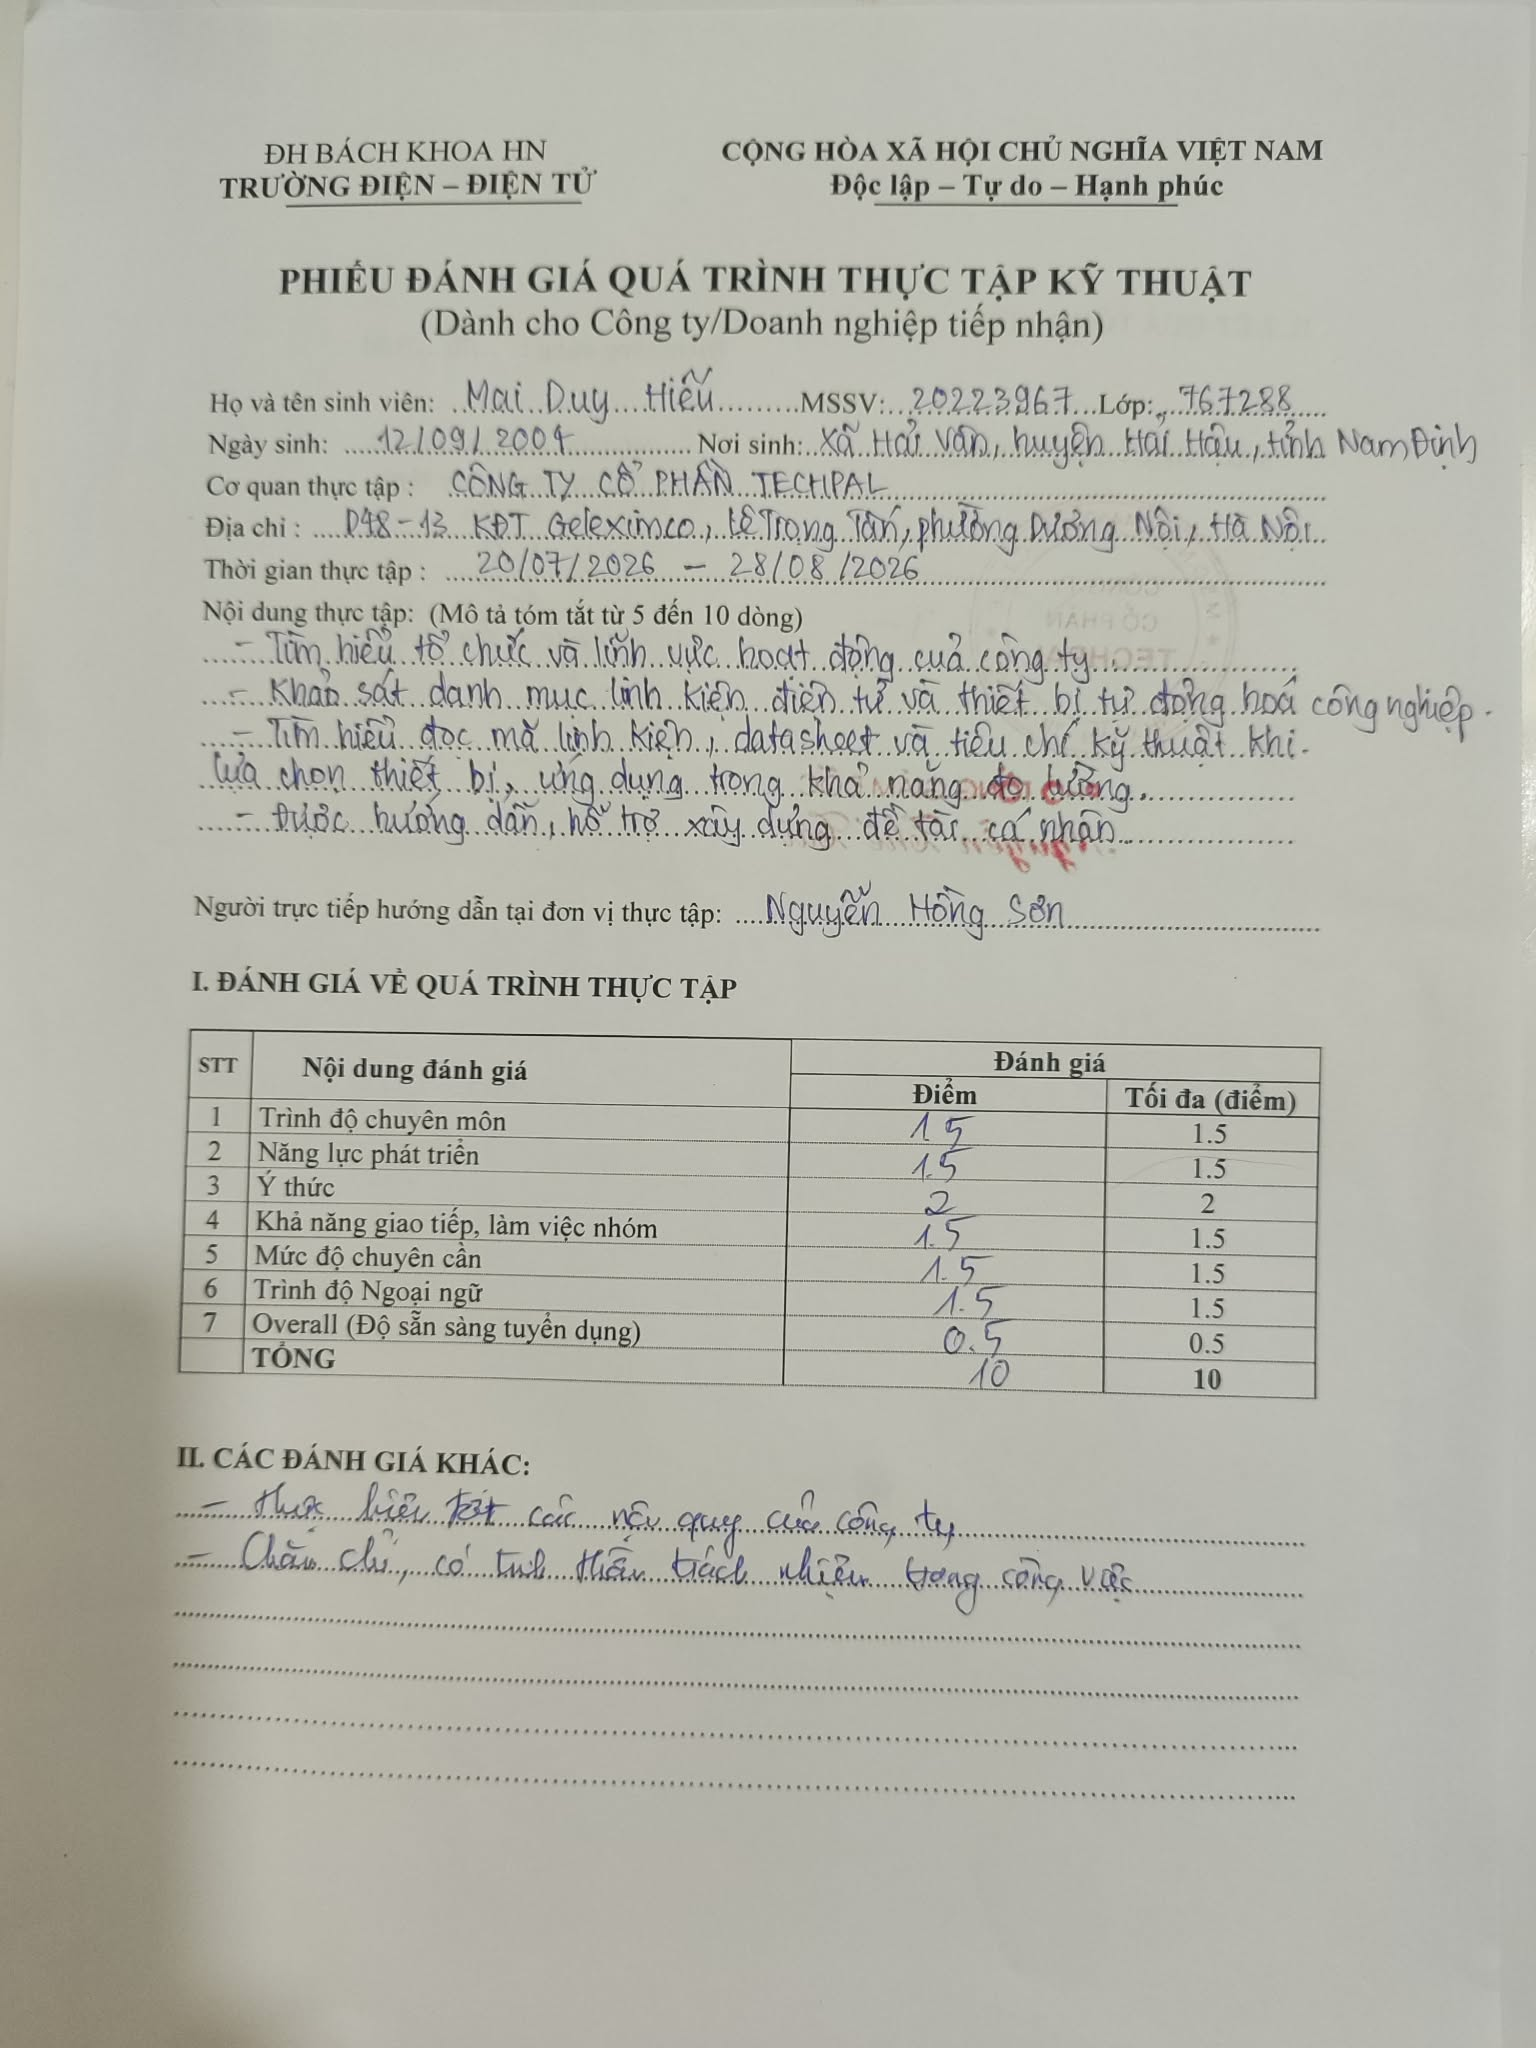
\includegraphics[width=0.82\textwidth]{phieu-danh-gia-trang-1.jpg.png}
\caption{Phiếu đánh giá quá trình thực tập (trang 1)}
\label{fig:phieu-trang-1}
\end{figure}

\begin{figure}[H]
\centering
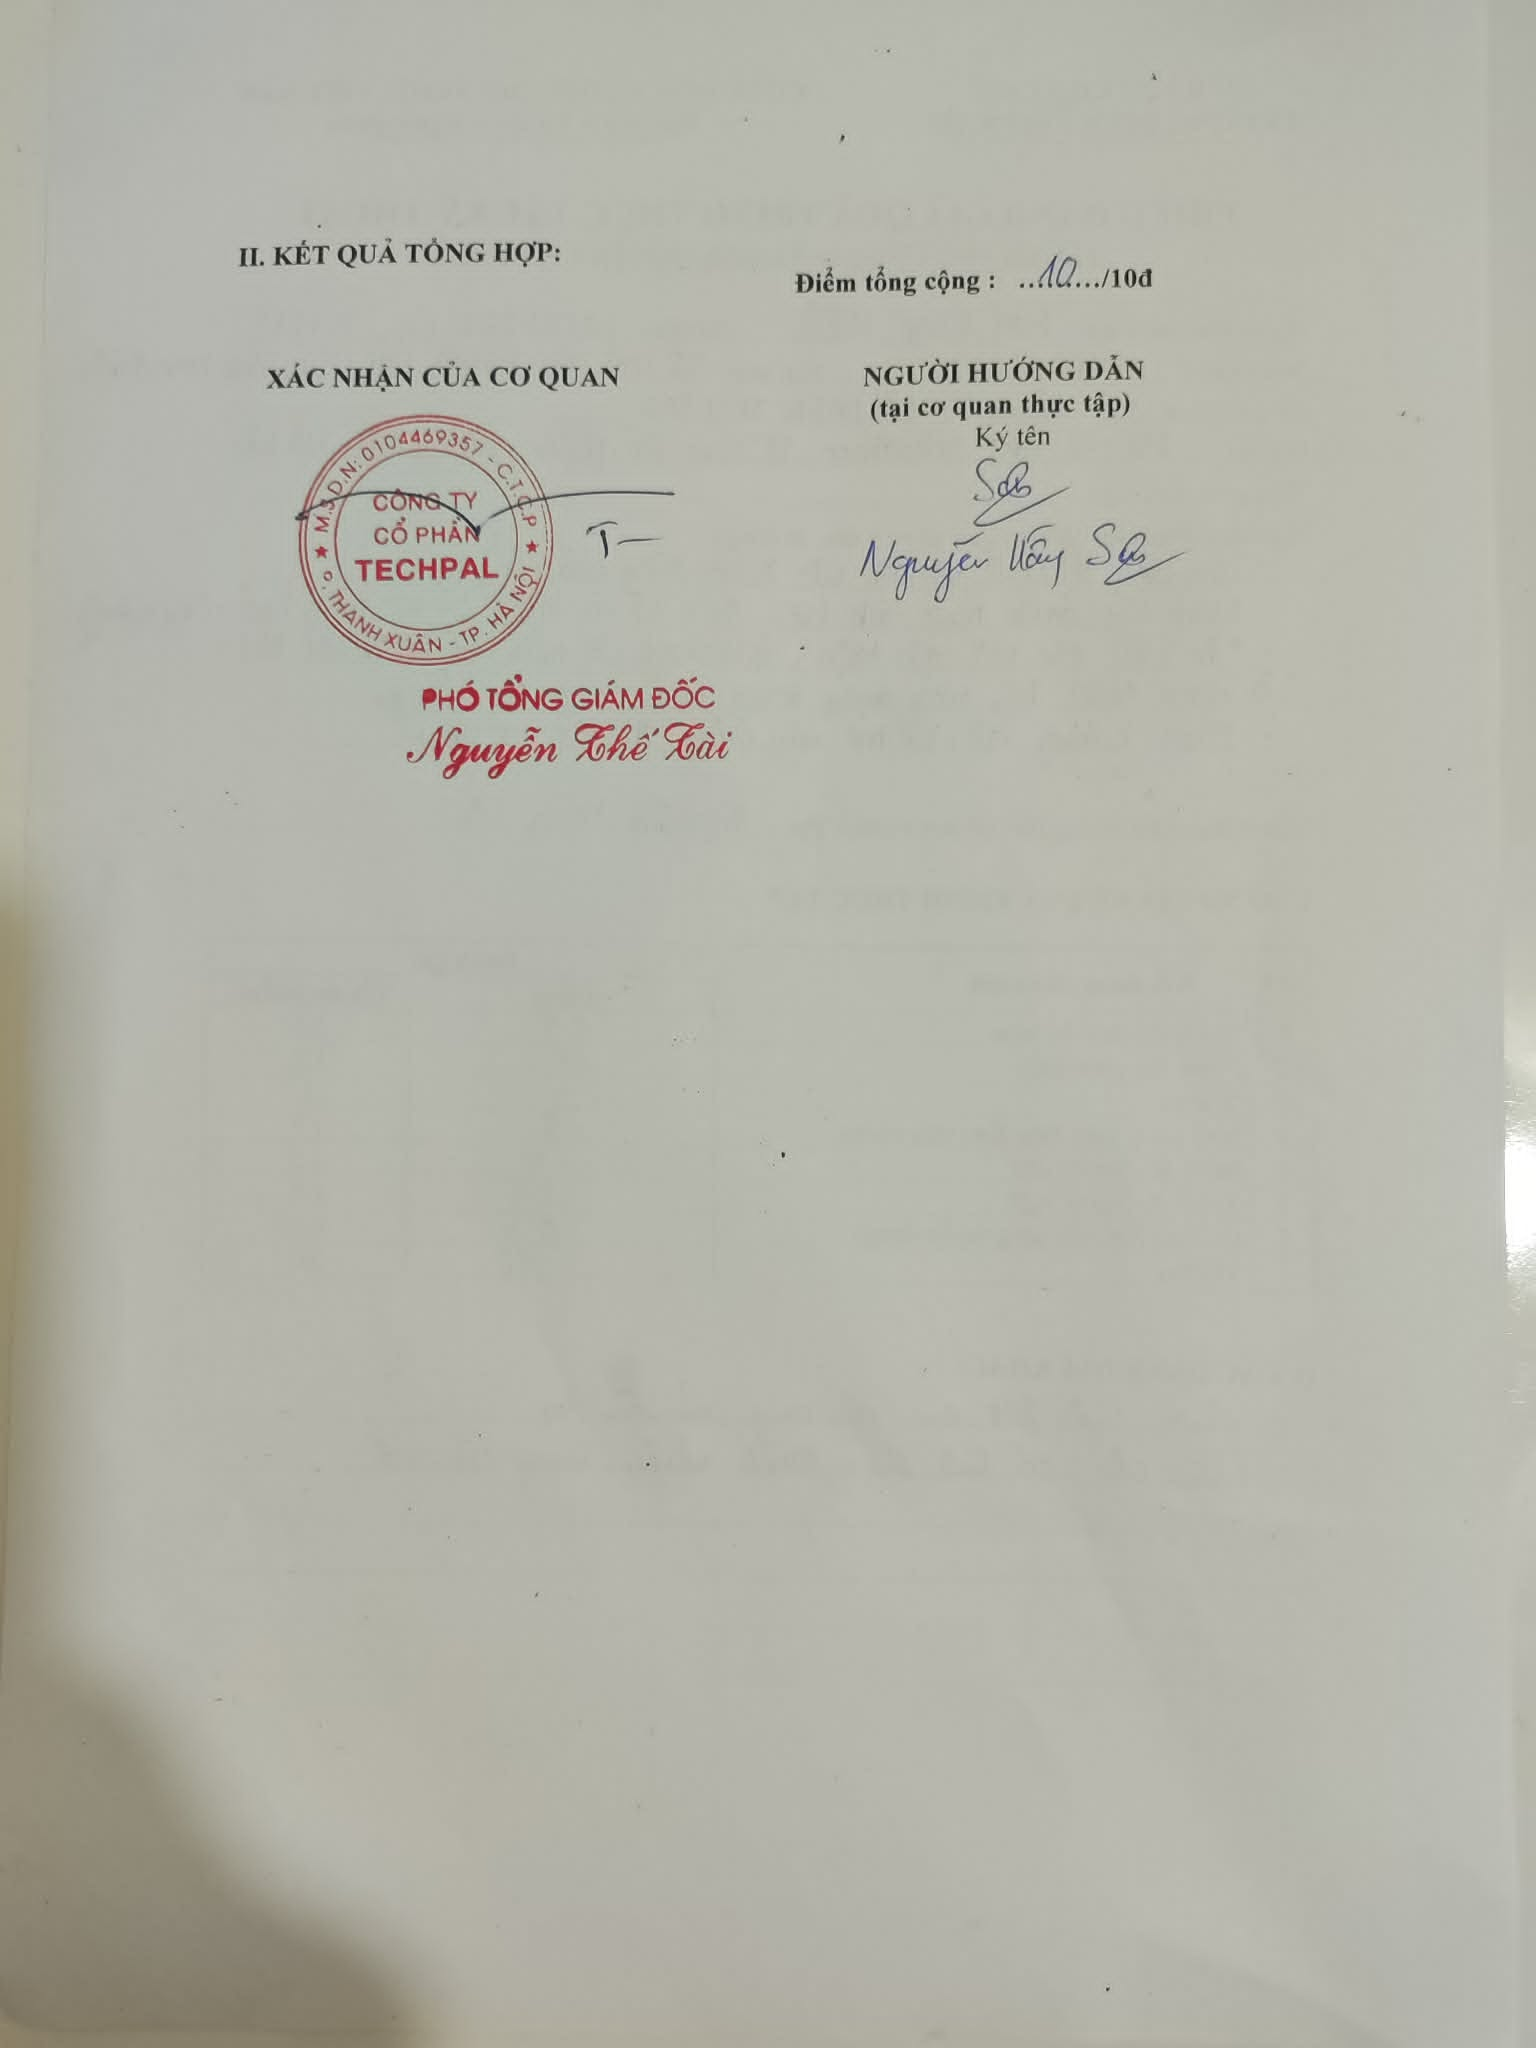
\includegraphics[width=0.82\textwidth]{phieu-danh-gia-trang-2.jpg.png}
\caption{Phiếu đánh giá quá trình thực tập (trang 2)}
\label{fig:phieu-trang-2}
\end{figure}
